\documentclass[]{revtex4-1}

\usepackage[fleqn]{amsmath}
\usepackage{amssymb,amsthm}
\usepackage[dvips]{graphicx}
\usepackage{color}
\usepackage{tabularx}

\newcommand{\recheck}[1]{{\color{red} #1}}
\newcommand{\redc}[1]{{\color{red} #1}}
\newcommand{\bluec}[1]{{\color{blue} #1}}
\newcommand{\greenc}[1]{{\color{green} #1}}
\newcommand{\vect}[1]{\textbf{\textit{#1}}}
\newcommand{\dd}[1]{\textsf{#1}}
\newcommand{\fwd}[0]{\textrm{fwd}}
\newcommand{\bwd}[0]{\textrm{bwd}}
\newcommand{\period}[0]{T_{\textrm{P}}}

\begin{document}


Dear Editor,\\

Below you find our reply to the the referees. We apologize for the long time needed for the reply due to the holiday of one of the authors.  The request of the referees implied a rather massive additional computational effort. The result of such effort is highly satisfactory and the validity of the paper is now much higher. We are now confident that the paper can be accepted for publication.\\

Best Regards\\


Han Wang (on behalf of all authors) 
\section*{Reply to referee 1}

\emph{On a principle level I am not sure that the relevant scientific
  question is really the non-equilibrium response since the response
  to the external field -- as the authors note -- is indeed quite
  fast. In fact, most of the discussion in the paper is focused on
  what I think could have been extracted just as well from
  conventional equilibrium simulations (conformational shifts,
  kinetics).}\\

We understand the concern of the referee and in the revised version of our manuscript have performed a numerical test.

We have employed equilibrium simulations to obtain the non-equilibrium
responses within the framework of linear responses theory (Green-Kubo relation).
With this approach we studied the conformational shift of alanine dipeptide under the electric field
(EF). As response function we have considered the time-dependent probability of
left-handed $\alpha$-helix (Conformation $C$ in the old manuscript. The notation has been changed to $\alpha_L$ in the updated manuscript.) This is defined as
\begin{align}\label{eqn:tmp1}
  P_C(t) = \langle\chi_{_C}(t)\rangle = \langle \chi_{_C} \rangle_0 -
  \beta \int_0^t ds\; M_e(t - s)\langle j(0)\cdot \chi_{_C}(t) \rangle_0
\end{align}
where $\chi_{_C}$ is the characteristic function of set $C$ that takes
the value of 1 for $(\phi,\psi)\in C$, and takes value 0
otherwise. $M_e(t)$ is the magnitude of the EF. In the case of
constant EF, $M_e(t) = t/t_{warm}$ for $0\leq t<t_{warm}$, and
$M_e(t) = 1$ for $t\geq t_{warm}$.
$j$ is the dissipative flux that is defined by
\begin{align}
  j = - \sum_{i=1}^N E_\infty q_i v_{i,x},
\end{align}
where $q_i$ is the partial charge of the $i$th atom, and $v_{i,x}$ is
the $x$ component of the velocity of the $i$th atom.  The notation
$\langle\cdot\rangle_0$ denotes the equilibrium ensemble average.
 We then plot the correlation function
$\langle j(0)\cdot \chi_{_C}(t) \rangle_0$ against correlation time $t$
in Fig.~\ref{fig:tmp1}~(a) of this reply. The value of the function is estimated from
two independent equilibrium simulations, and the trajectory of each is
of 1~$\mu$s. The total length of the equilibrium
trajectories is the same as the non-equilibrium simulation (2000
trajectories, each 1000~ps long).
We find that the statistical error is even larger than the value of
correlation function.
In Fig.~\ref{fig:tmp1}~(b),
  the probability of conformation $C$ calculated from
  the linear response theory is compared with that
  computed from non-equilibrium simulation.
  The linear response result follows the non-equilibrium result only in the very first
  15~ps, then it diverges. Since it is meaningless for a probability
  being larger than 1, the linear response result is qualitatively wrong.
Therefore, the
overwhelming statistical uncertainty does not suggest to use the equilibrium approach 
in Eq.~\eqref{eqn:tmp1} to calculate the
non-equilibrium averages. 
% , and we actually do not know when the
% corrlation function vanish .
Since the total computational effort of
the equilibrium simulation is the same as the non-equilibrium
simulation, we conclude that non-equilibrium simulation is more
accurate and efficient than the conventional equilibrium approach  at the same computational cost.
It must be noticed that a similar
observation has already been reported by Ciccotti and Jacucci, (Phys.~Rev.~Lett.~35, 789, 1975). We report the description above in the appendix of the manuscript.
\\
\begin{figure}
  \centering
  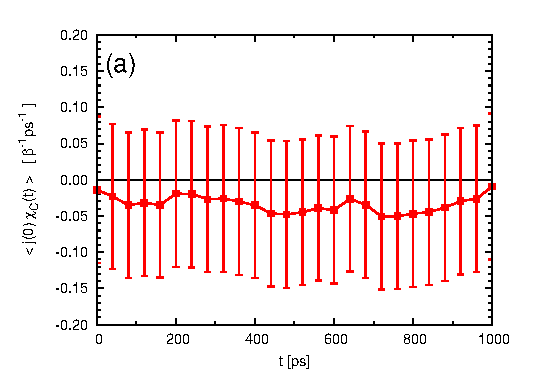
\includegraphics{figs/fig-corr-meta.eps}
  \includegraphics{figs/fig-corr-meta-c.eps}
  \caption{
    The numerical result of the linear response theory.
    (a): The correlation function $\langle j(0)\cdot \chi_{C}(t)
    \rangle_0$ against time $t$.
    The error bars in the figure denote
    the statistical uncertainty at 95\% confidence level. 
    (b): The probability of conformation $C$ computed from the
    linear response theory versus that
    computed from non-equilibrium simulation (D-NEMD).}
  \label{fig:tmp1}
\end{figure}


\emph{
In the alanine dipeptide system studied here, I am not sure that the
initial simulation is in fact fully converged and -- if the question is
how conformational preferences evolve in response to an external field
-- whether the short branch simulations are long enough to establish
convergent sampling. More specifically, I think that the lack of
sampling of the left-handed helix in the absence of an electric field
is a result of insufficient sampling to cross the kinetic barrier from
beta to alphaL conformations (alanine dipeptide with CHARMM27 has been
extensively characterized and I suggest a comparison with relevant
papers from MacKerell et al.). If such relevant conformations are
missing from the initial snapshots and the branch simulations are
short I am concerned that the resulting initial bias affects the
non-equilibrium results.
}\\

We have done an equilibrium simulation of 1~$\mu$s.  Along the
trajectory, molecular conformations are recorded every 500~ps,
therefore, in total 2000 equilibrium conformations are extracted.  The
equilibrium probabilities of the conformations $A_1$, $A_2$, $B_1$,
$B_2$ and $C$ are 0.426 ($\pm 0.029$), 0.076 ($\pm 0.010$), 0.265
($\pm 0.013$), 0.182 ($\pm 0.019$) and 0.051 ($\pm 0.021$),
respectively.  We run two additional equilibrium simulations of
1~$\mu$s, and the probabilities of conformations are consistent with
the values listed above, which means that our ``new'' equilibrium
simulation is fully converged.  Comparing with our previous
equilibrium simulation (only 0.1~$\mu$s long),
% in which the
% probability of left-handed $\alpha$-helix is only 0.008,
the precision
of initial configuration sampling is substantially improved. All
simulations in the manuscript are re-performed according to the new set
of initial conformations, however nothing substantially changed compared to the original results.\\

We have also tested the convergence of simulation results with respect to the
number of branching trajectories.  The time-dependent probabilities of
each conformation calculated from one branching trajectory is compared
with four branching trajectories (each of them is simulated with
different random seeds for Langevin thermostat) in
Fig.~\ref{fig:tmp2} of this reply. The results are consistent with the original ones, which means that the
sampling of the non-equilibrium trajectories is fully converged. In
summary, since our non-equilibrium simulation includes the
sampling of both initial configurations and non-equilibrium
trajectories, the convergence of both  implies the convergence
of our simulation results. 
The updated results are added in the paper.\\

The question on whether our non-equilibrium branching trajectories are
long enough so that the results are fully converged is an always present problem. There may exists an intrinsic time-scale longer than our simulation time, however this is obvious and implicitly imply that the validity of our results is restricted to the time scale simulated. 
\\

\begin{figure}
  \centering
  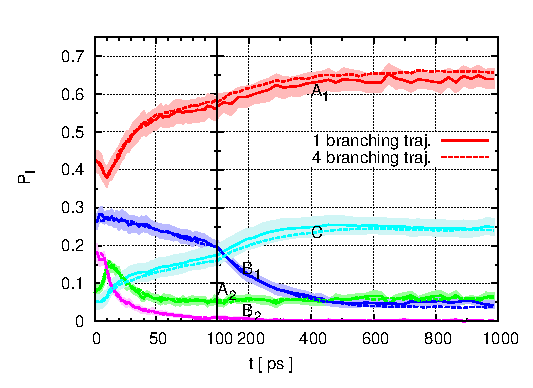
\includegraphics{figs/fig-meta-more.eps}
  \caption{A comparison between the simulation with one branching
    trajectory per every initial conformation and four branching
    trajectories  for the
    constant EF case. Each of the four
    branching trajectories is simulated with a different random seed for
    Langevin thermostat.
    The shadow region presented with each line of the one-branching-trajectory case
    denotes its statistical uncertainty at 95\% confidence level.  }
  \label{fig:tmp2}
\end{figure}

\emph{ It looks as if the CMAP correction was used with the CHARMM
  force field but no information is given in the methods section.}\\

Yes, the CMAP correction is used. We mention it in the
section III.A. of the updated manuscript.
\\

\emph{
I am curious how the choice of Rex for the thermostat would affect the
results.
}\\

We compared the simulation results of two different $R_{ex}$ values:
1.0~nm and 1.5~nm in Fig.~7 (pp.15) of the manuscript. The
$R_{ex}=1.0$~nm case was simulated in periodic cubic simulation box
of length $L=2.7$~nm and 4.0~nm.  The $R_{ex}=1.5$~nm case was
simulated in cubic box of length $L=4.0$~nm. Fig.~7 of the
manuscript demonstrates that all the results are consistent. This
means $R_{ex}=1.0$~nm is already large enough, and a larger $R_{ex}$
would not change the results.\\

\emph{ I wonder about the motivation of using electric fields with
  periods of 10, 40, and 200ps. How do such fields relate to the
  practical question of electromagnetic radiation exposure?  }\\

The periods 10, 40~ps are roughly the same as the first two shortest
time scales of probability fluxes observed in the constant EF case,
see Table~I of the manuscript. We tried to do a simulation with period of
500~ps, which is the same as the longest timescales of the constant EF
case, however, the required simulation time is prohibitive at this stage. Therefore, we made a reasonable compromise and considered only
a period of 200~ps. The typical frequency of the microwave
irradiation is 2450~MHz, which corresponds to period of 400~ps. It is
the same order of magnitude as the $T_P=200$~ps studied by us.
We have added a comment along these lines in the revised manuscript.
\\

\emph{ The analysis of ``probability fluxes'' seems to be nothing else
  than a kinetic analysis. Maybe some comments on how these are
  related would be helpful.  }\\

Yes, the definition of the probability fluxes is similar to the
kinetic rate (we use joint probabilities in (6) rather than
conditional probabilities).
However, we prefer to stick to our definition which
is mathematically simpler and univocal.
A comment along this direction has been added to the end of section III.B.
\\
% However, we want to stress out that, in general,
% the probability fluxes calculated in the manuscript should not be
% interpreted as a kinetic rate, and one cannot replace the
% non-equilibrium molecular dynamics by a kinetic analysis. The main
% reasons are:
% Firstly, for a non-equilibrium system, the probability fluxes are
% time-dependent, therefore, the lag-time $\Delta t$ in the definition (Eq.~(6))
% should be small compared with the typical time-scale of conformation change.\\
% Secondly, for a small lag time $\Delta t$ (1~ps in the manuscript), the conformational
% dynamics of biomolecules is generally not
% Markovian (see e.g.~C.~Sch\"utte et.~al.~JCP 2011 and J.-H.~Prinz et.~al.~JCP 2011).
% Since the basic assumption -- Markovianity -- of the kinetic analysis
% may not be satisfied, a direct
% application of the kinetic analysis in the non-equilibrium cases is questionable. Although one may
% gain useful information from the kinetic analysis, the reliability
% and the effectiveness of this approach should be carefully checked case
% by case.  Since the main goal of our research is to propose a
% non-equilibrium molecular dynamics simulation method, the numerical
% results are not compared with a kinetic analysis.\\


\emph{Finally, given the apparent convergence issues with alanine
  dipeptide I have difficulties seeing how this method could be
  applied in a reasonable manner to more complex systems. Maybe some
  comments to that extent would be helpful.  }\\


The referee is invited to look at the reply to the second question concerning the convergence
of our simulation results. We believe that a better initial
state sampling and the new convergence check with respect to the
number of branching trajectories will strengthen the reliability
of our method.
% manuscript and



% We have added a section in the appendix in the manuscript discussing
% the convergence and reliablity of our method. Please also see the
% answer to the 2nd question.



\section*{Reply to referee 2}

\emph{
It would be useful if the authors would briefly comment on the
relationship between time-varying electric fields and terahertz
spectroscopy. Experimental work in this frequency range may be related
directly to the results reported here. See work by Plusquellic et al
(ChemPhysChem 2007), Havenith et al. (Faraday 2009) and others.
}\\

The frequencies investigated in our manuscript span from 5~GHz to 100~GHz,
the largest of which is still one order of magnitude smaller than those normally used in  terahertz spectroscopy. Therefore, we find that our simulation results, at this stage, cannot be directly compared with the terahertz experiments.
{To make fully aware the readers about the current limitation of our study, with respect to experimental connections, we have added the comment above and the experimental references in the manuscript.}
\\

\emph{ The procedure for controlling the temperature under neq
  conditions is reminiscent of the ``stochastic boundary conditions''
  introduced by Brooks and Karplus (JCP 1983). Can the authors provide
  a more formal description of their procedure and touch on
  similarities/dissimilarities with the Brooks/Karplus approach?  }\\

Yes, a comment and comparison along this direction has been added to the
manuscript.\\

\emph{ In the methods sections the treatment of H-involving bonds is
  not explained (SHAKE, RATTLE, ??). Also, a reference for the TIP3P
  model should be given. What cutoffs are required for an "energy
  conserving PME" simulation and how were the vdw interactions
  handled?  }\\

The asked details has been added to the manuscript.\\

\emph{
It is suggested to adapt the labeling of the conformational substates
of alanine dipeptide to that used in the literature ($C7_{eq}$, $\alpha_L$,
$C7_{ax}$, etc.) - see e.g. Caflisch et al., JCP 1999.
}\\

We have changed the labeling of conformations.\\

\emph{
The sentence ``..how the behaviour of the electric dipole moment of the
molecule is influenced..'' reads somewhat strange. Obviously, each of
the metastable states has its own dipole moment and this is reported
later on p. 12. However, there is no reason why the EF should
\emph{influence} the dipole moment as the simulations employ a force field
with fixed charges. It would probably be helpful to clarify that the
EF leads to ``conformational selection'' through alignment of the
molecular dipole along the EF.
}\\

We have made corresponding changes to the manuscript.\\

\emph{ It would be interesting to relate the probability fluxes from
  Fig 11 to the work by Rao et al. (PNAS 2007) and the Caflisch JCP
  1999 article. It should be possible to relate the probability fluxes
  to free energy differences.}\\

This is indeed a very interesting point.
Although the network presented in Fig.11 is similar to those
discovered in the mentioned equilibrium studies,
regarding the map of the steady conformations and connections among them,
the physical meaning is instead quite different in our study:
The system is under nonequilibrium conditions, and
the fluxes are explicitly induced by a physically realistic control, i.e.~EF, although the averaged population of the steady conformations do not change. In contrast,
such probability fluxes do not exist, as a result of an explicit physical action, in the equilibrium case.
A comment along such direction has been added to the
manuscript.\\

% It must be also added that the transition fluxes can be used to calculate the free energy only in
% the equilibrium case. In the non-equilibrium case, especially for the
% oscillatory EF case, the conformational kinetics of the system is generally
% not Markovian. Therefore, the standard kinetic analysis cannot be used
% here.

\end{document}
